\documentclass[border=10pt]{standalone}
\usepackage[svgnames]{xcolor}
\usepackage{amsmath}
\usepackage{pgfplots}
\pgfplotsset{compat=newest}
\usepackage[sfdefault]{FiraSans}
\usepackage{FiraMono}
\renewcommand*\familydefault{\sfdefault}
\begin{document}
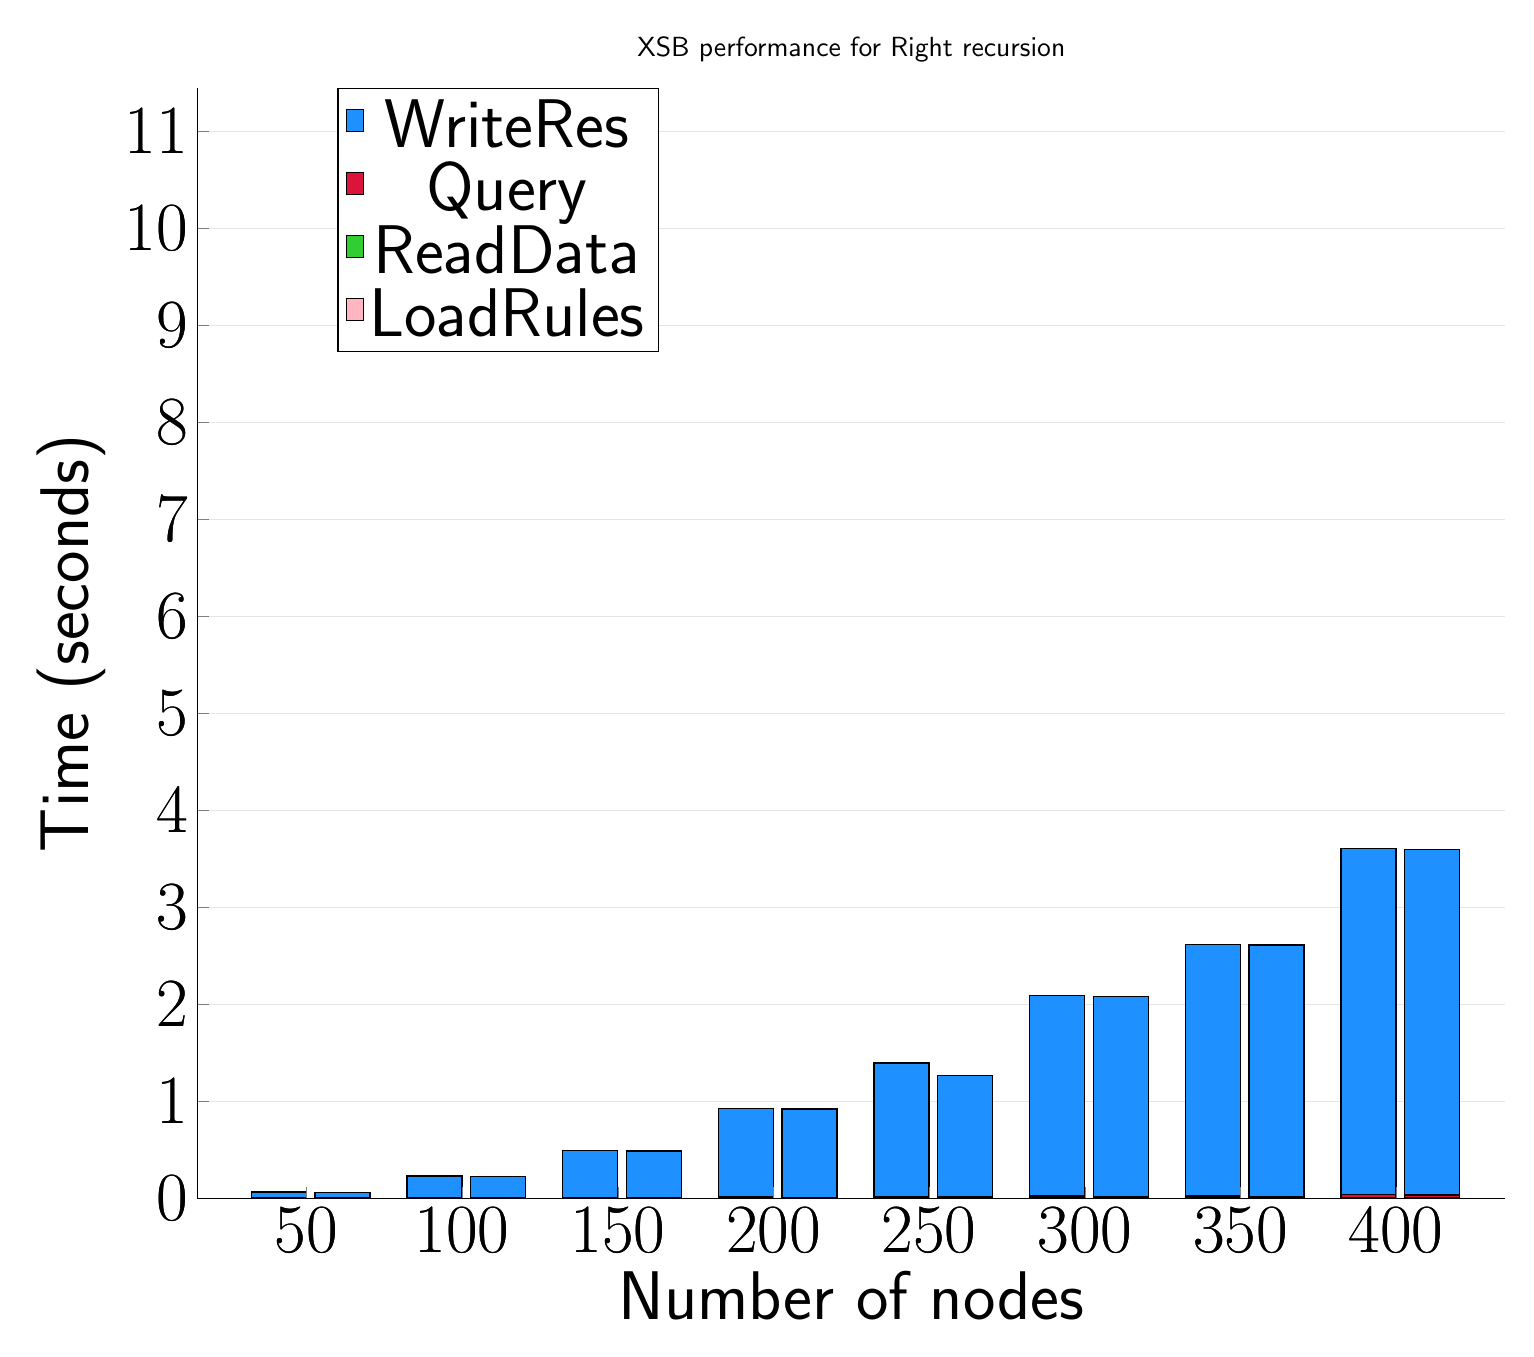
\begin{tikzpicture}
\begin{axis}[
   ybar stacked,
   title={XSB performance for Right recursion},
   bar shift=-10pt,
   width=1.5\textwidth,
   bar width=0.7cm,
   ymajorgrids, tick align=inside,
   major grid style={draw=gray!20},
   xtick=data,
   ymin=0, ymax=11.449559211730957,
   axis x line*=bottom,
   axis y line*=left,
   enlarge x limits=0.1,
   legend style={
       at={(0.23, 1)},
       anchor=north,
       legend columns=1,
       font=\Huge,
   },
   ylabel={Time (seconds)},
   xlabel={Number of nodes},
   label style={font=\Huge},
   tick label style={font=\Huge},
]
\addlegendimage{fill=DodgerBlue, draw=black, line width=0.2pt}
\addlegendentry{WriteRes}
\addlegendimage{fill=Crimson, draw=black, line width=0.2pt}
\addlegendentry{Query}
\addlegendimage{fill=LimeGreen, draw=black, line width=0.2pt}
\addlegendentry{ReadData}
\addlegendimage{fill=LightPink, draw=black, line width=0.2pt}
\addlegendentry{LoadRules}
\addplot +[fill=LightPink, draw=black, line width=0.5pt] coordinates {
    (50, 0.005399306615193686)
    (100, 0.0048389434814453125)
    (150, 0.00485531489054362)
    (200, 0.004567941029866536)
    (250, 0.004197359085083007)
    (300, 0.004640897115071613)
    (350, 0.004688580830891926)
    (400, 0.005212942759195964)
};
\addplot +[fill=LimeGreen, draw=black, line width=0.5pt] coordinates {
    (50, 0.0018575986226399735)
    (100, 0.0026267369588216134)
    (150, 0.0033700466156005838)
    (200, 0.003765344619750977)
    (250, 0.004218101501464844)
    (300, 0.00504342714945475)
    (350, 0.005818367004394534)
    (400, 0.008214712142944336)
};
\addplot +[fill=Crimson, draw=black, line width=0.5pt] coordinates {
    (50, 0.00043503443400065095)
    (100, 0.0016500155131022166)
    (150, 0.00353264808654785)
    (200, 0.006028652191162107)
    (250, 0.007770538330078126)
    (300, 0.016385952631632467)
    (350, 0.016436338424682635)
    (400, 0.025560935338338236)
};
\addplot +[fill=DodgerBlue, draw=black, line width=0.5pt] coordinates {
    (50, 0.05892332394917804)
    (100, 0.2217133839925128)
    (150, 0.48380899429321317)
    (200, 0.9119044144948322)
    (250, 1.3814984162648554)
    (300, 2.0659693876902243)
    (350, 2.5911950270334874)
    (400, 3.568543752034509)
};
\end{axis}
\begin{axis}[
   ybar stacked,
   bar shift=13pt,
   width=1.5\textwidth,
   bar width=0.7cm,
   ymajorgrids, tick align=inside,
   major grid style={draw=none},
   xtick=data,
   ymin=0, ymax=11.449559211730957,
   axis x line*=none,
   axis y line*=none,
   enlarge x limits=0.1,
   label style={font=\Huge},
   tick label style={font=\Huge},
]
\addplot +[fill=LightPink, draw=black, line width=0.5pt] coordinates {
    (50, 0.005147000000000003)
    (100, 0.004241333333333334)
    (150, 0.004157)
    (200, 0.0044856666666666664)
    (250, 0.003969333333333333)
    (300, 0.0039840000000000006)
    (350, 0.003310000000000006)
    (400, 0.005212666666666664)
};
\addplot +[fill=LimeGreen, draw=black, line width=0.5pt] coordinates {
    (50, 0.0017709999999999965)
    (100, 0.002603)
    (150, 0.002866)
    (200, 0.0037383333333333366)
    (250, 0.004202999999999997)
    (300, 0.0050156666666666665)
    (350, 0.005759666666666663)
    (400, 0.00821766666666667)
};
\addplot +[fill=Crimson, draw=black, line width=0.5pt] coordinates {
    (50, 0.0004149999999999983)
    (100, 0.0016509999999999969)
    (150, 0.003371666666666663)
    (200, 0.004230999999999996)
    (250, 0.0077726666666666664)
    (300, 0.013575666666666666)
    (350, 0.014156666666666666)
    (400, 0.02208033333333333)
};
\addplot +[fill=DodgerBlue, draw=black, line width=0.5pt] coordinates {
    (50, 0.053276333333333335)
    (100, 0.216944)
    (150, 0.479125)
    (200, 0.9122843333333334)
    (250, 1.2498573333333332)
    (300, 2.0578766666666666)
    (350, 2.5914103333333336)
    (400, 3.565314666666667)
};
\end{axis}
\end{tikzpicture}

\end{document}
